\chapter{Všeobecný prehľad a teória}\label{chap:teoria}

Umelá inteligencia (UI) zaznamenala za posledných niekoľko desaťročí obrovský rast a vývoj, ktorý posunul hranice možností počítačov. Na čele UI je oblasť počítačového videnia využívajúca konvolučné neurónové siete, ktoré dosahujú prelomové výsledky v úlohách rozpoznávania obrazov a objektov. 

Na to aby sme vedeli vygenerovať úrovne pre rytmické počítačové hry, musíme najprv porozumieť, čo sú to rytmické počítačové hry a ako fungujú, a zároveň musíme porozumieť, ako fungujú neurónové siete a ako ich môžeme použiť na generovanie úrovní. V tejto kapitole sa budeme venovať týmto témam a zároveň sa budeme venovať aj teórii, ktorá je potrebná na pochopenie tejto práce.

\section{Rytmické Počítačové Hry a Ich Štruktúra}\label{sec:rytmicke_hry}


Rytmické počítačové hry predstavujú špecifický žáner videohier, kde je kľúčovým aspektom hrateľnosti hudba a rytmus. Hráči v týchto hrách nie sú len pasívnymi pozorovateľmi, ale aktívne interagujú s herným prostredím, pričom ich akcie sú synchronizované s hudobnými prvkami. V týchto hrách hráči často vykonávajú preddefinované akcie, ako sú stlačenia kláves alebo tlačidiel v rytmickom poradí, v súlade s hudbou a vizuálnymi indikáciami na obrazovke.

Kľúčové charakteristiky rytmických počítačových hier zahŕňajú:

\begin{itemize}
\item \textbf{Hudobný Prvok} – Hudba nie je len pozadím, ale aktívne ovplyvňuje hrateľnosť a vizuálny dizajn hry. Hráči reagujú na hudobné prvky, ako sú rytmus a melódia.
\item \textbf{Vizuálne Indikácie} – Na obrazovke sa zobrazujú grafické indikácie alebo symboly, ktoré signalizujú hráčovi, kedy a aké akcie je potrebné vykonať. Vizuálne prvky sú synchronizované s hudobným pozadím.
\item \textbf{Preddefinované Akcie} – Hráči vykonávajú preddefinované akcie, ako sú stlačenia kláves alebo tlačidiel, v súlade s hudbou a vizuálnymi indikáciami na obrazovke.
\item \textbf{Úrovne alebo Levely} – Hry často obsahujú štruktúrované úrovne alebo levely, kde sa obtiažnosť postupne zvyšuje. Hráči dosahujú úspech tým, že dokončujú úrovne s vysokou presnosťou a bodovým skóre.
\end{itemize}

Tieto hry nie len poskytujú zábavu, ale tiež stimulujú hráčové vnímanie hudby a rytmu, vytvárajúc jedinečný zážitok spojením digitálnej zábavy s hudobným umením.

\section{Rôzne typy rytmických počítačových hier}\label{sec:typy}


Rozlíšenie medzi rôznymi typmi rytmických hier môže byť užitočné na porozumenie rôznych prístupov k tomuto žánru. Tu sú niektoré základné typy rytmických hier a ich charakteristiky:

\begin{itemize}

\item \textbf{Tanečné hry} – Hráči tancujú na hudbu a snažia sa napodobniť tanečné kroky, ktoré sú zobrazené na obrazovke, poprípade majú tanečnú podložku, na ktorej sa nachádzajú tlačidlá, na ktoré je potrebné stúpiť keď sa na obrazovke. Príkladom tanečných hier sú \textit{Just Dance} alebo \textit{Dance Dance Revolution}.
\item \textbf{Hry s Nástrojmi} – Hráči hrajú na reálne hudobné nástroje, ako sú gitara alebo klávesy. Hráči musia zahrať správne tóny v správnom čase. Príkladom hier s nástrojmi sú \textit{Guitar Hero} alebo \textit{Rock Band}.
\item \textbf{Hry s Dotykovým Displejom} – Hráči stláčajú tlačidlá alebo podobné objekty na dotykovom displeji. Príkladom hier s dotykovým displejom sú \textit{Beatstar} alebo \textit{osu!}.
\item \textbf{Hry vo Virtuálnej Realite} – Hráči interagujú s rôznymi objektami v hernom prostredí vo virtuálnej realite. Príkladom hry vo virtuálnej realite je \textit{Beat Saber}.
\end{itemize}

Poslednému zmieňovanému typu a hre \textit{Beat Saber} sa budeme venovať v tejto práci. 

\section{Hra Beat Saber}\label{sec:beat_saber}

Beat Saber je hra pre virtuálnu realitu, ktorá bola vyvinutá a vydaná českým herným štúdiom Beat Games. Hra bola v predbežnom prístupe vydaná v máji 2018 a neskôr v máji 2019 bola vydaná ako plná verzia. Hra je dostupná pre platformy PlayStation 4, Windows, Meta Quest a ďalšie. Hráč používa ovládače pre virtuálnu realitu na ovládanie dvoch svetelných mečov, ktoré sú prednastavené na červenú a modrú farbu pre ľavú a pravú ruku. \cite{sutrich2020beatsaber}

V každej pesničke hra hráčovi predkladá postupnosť približujúcich sa blokov súčasne s rytmom hudby, umiestnených v jednej z 12 možných pozícií na mriežke 4×3. Každý blok môže byť označený šípkou, ktorá naznačuje jednu z ôsmich možných smerov, ktorým musí byť blok správne pretnutý. Existujú aj bloky s bodkami namiesto šipiek, ktoré hráči môžu zasiahnuť z akéhokoľvek smeru. Okrem toho sa objavujú aj bomby, ktoré hráč nesmie zasiahnuť, a prekážky v podobe približujúcich sa stien, ktorým sa je potrebné vyhnúť hlavou.

Beat Saber bol dodaný s desiatimi piesňami, ale bol rozšírený niekoľkými balíkmi s obsahom na stiahnutie a aktualizáciami, ktoré zahŕňajú nové piesne. Niekoľko z nich obsahuje originálne skladby, ale niekoľko balíkov obsahuje licencované piesne s hudbou a špeciálnymi úrovňami od rôznych umelcov. Okrem toho komunita vytvorila modifikácie pre Beat Saber, ktoré umožňujú vlastné piesne a mapy.

Počas hry sa objavujú bloky, ktoré majú rôzne špeciálne efekty, ako napríklad blok s vedenou čiarou alebo blok pozostávajúci z viacerých menších blokov. Zároveň má hra veľmi bohato editovateľné vizuálne efekty, ako napríklad laserové show a podobne. V aktuálnej verzii hry sú k dispozícii 5 rôznych herných režimov: Standard, No Arrows (bloky je možné pretnúť v akomkoľvek smere), One Saber (používa sa len jeden meč), 90 Degrees a 360 Degrees (bloky sa približujú v rôznych smeroch).

Hra má tiež niekoľko úrovní obtiažnosti, ktoré sú Easy, Normal, Hard, Expert a Expert+. Tieto úrovne obtiažnosti sa líšia počtom blokov, rýchlosťou približovania sa blokov, počtom prekážok a podobne.

V našej práci sa budeme venovať režimu Standard, ktorý je najpoužívanejší a najviac rozšírený. A zároveň sa budeme venovať trom základným objektom v hre, ktorými sú bloky, prekážky a bomby (vyobrazených na Obr. \ref{fig:blocks}). Zameriame sa aj na všetky úrovne obtiažnosti, ktoré sú dostupné v hre.

\begin{figure}[H]
  \centerline{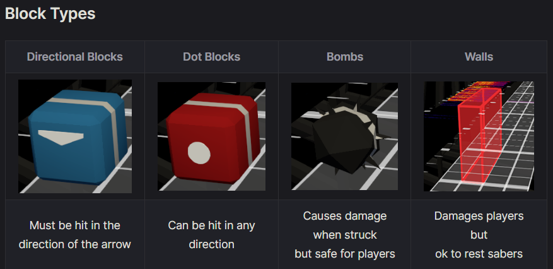
\includegraphics[width=0.75\textwidth]{images/block types.png}}
  \caption{Ukážka blokov, prekážok a bômb v hre Beat Saber. (Zľava – smerovací blok, blok s bodkou, prekážka, bomba)}
  \label{fig:blocks}
  \end{figure}

\subsection{Tvorba Chart Súborov pre Beat Saber}

Jedným z kľúčových prvkov, ktorý prispieva k úspechu tejto hry, sú chart súbory, ktoré vytvárajú komunitní tvorcovia. Chart súbory obsahujú informácie o pozíciách a časoch blokov, prekážok. Najpoužívanejším nástrojom na tvorbu chart súborov je ChroMapper. V tomto nástroji si načítame hudbu, ktorú chceme použiť, zadáme základne informácie o pesničke, ako názov, autora a podobne. Následne tvorca vyberie obtiažnosť (napr. \textit{Easy}) a typ mapy (napr. \textit{Standard}), ktorú chce vytvoriť. Potom sa načíta obrazovka, kde sa nachádza mriežka 4×3, kde sa nachádzajú pozície, kde sa budu vkladať zvolené objekty. Ukážku prostredia je možné vidieť na Obr. \ref{fig:chromapper}. Na vrchu obrazovky sa nachádzajú tlačidlá, ktorými sa vyberajú objekty.Na koniec, po vložení všetkých objektov, si tvorca uloží súbor a aplikácia vygeneruje všetky potrebné súbory, ktoré je možne následne načítať do hry.

\begin{figure}[H]
  \centerline{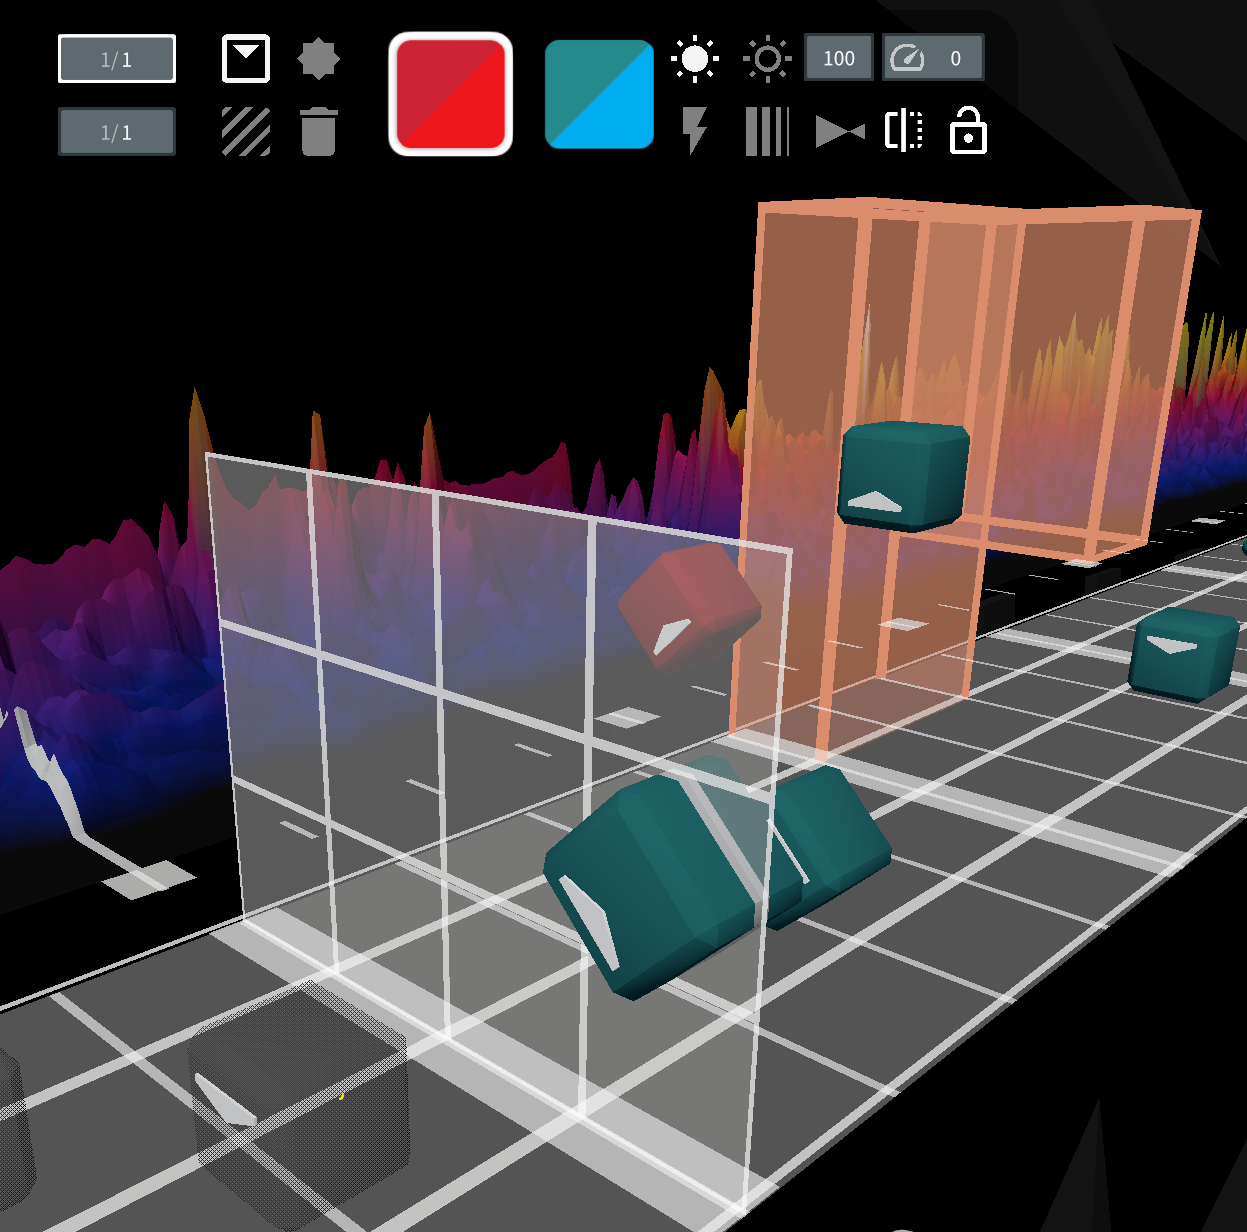
\includegraphics[width=0.5\textwidth]{images/chromapper.png}}
  \caption{Ukážka prostredia nástroja Chromapper.}
  \label{fig:chromapper}
  \end{figure}

\subsubsection{Kľúčové Aspekty Tvorby Chart Súborov}

Tvorba chart súborov je veľmi náročný proces, ktorý vyžaduje veľa času a ale ak skúseností. Chart súbory musia byť vytvorené tak, aby boli zábavné a zároveň výzvou pre hráčov. Tvorcovia musia zvážiť niekoľko kľúčových aspektov, aby sa zabezpečilo, že ich chart súbory budú zábavné a zároveň výzvou pre hráčov. Tu sú niektoré z týchto aspektov:

\begin{itemize}
\item \textbf{Priraďovanie Beatov a Blokov} – Tvorcovia musia zvážiť, ktoré beaty v hudbe budú priradené k blokom. Všeobecne platí, že beaty, ktoré sú v hudbe výraznejšie, by mali byť priradené k blokom. 
\item \textbf{Dynamika Pohybov Hráča} – Tvorcovia musia správne koncipovať pohyby a kombinácie blokov tak, aby boli intuitívne a plynulé pre hráča
\item \textbf{Nastavenie obtiažnosti} – Tvorcovia musia zvážiť, akú obtiažnosť chcú dosiahnuť. Všeobecne platí, že vyššia obtiažnosť znamená viac blokov a rýchlejšie pohyby.
\end{itemize}

\section{Trénovanie neurónových sietí}\label{sec:trenovanie_nn}

Na to aby sme vedeli vygenerovať úrovne, musíme porozumieť základným princípom neurónových sietí a ich trénovania. Zadefinujme si pojmy ako neurónová sieť, aktivačná funkcia, stratová funkcia a podobne.

\subsection{Neurónové Siete} \label{sec:neuronove_siete}

Neurónové siete sú modely strojového učenia, ktoré sú inšpirované biologickými neurónovými sieťami. Neurónové siete sa skladajú z viacerých vrstiev neurónov, ktoré sú navzájom prepojené. Tieto neuróny v sebe uchovávajú číselnú hodnotu. Neurónová sieť sa skladá z vstupnej a výstupnej vrstvy, medzi ktorými sa nachádzajú skryte vrstvy. Pokiaľ ma neurónová sieť viac ako dve skryte vrstvy, hovoríme o hlbokých neurónových siatiach. Ilustráciu hlbokých neurónových sietí môžeme vidieť na Obr. \ref{fig:neuron}.

\begin{figure}[H]
\centerline{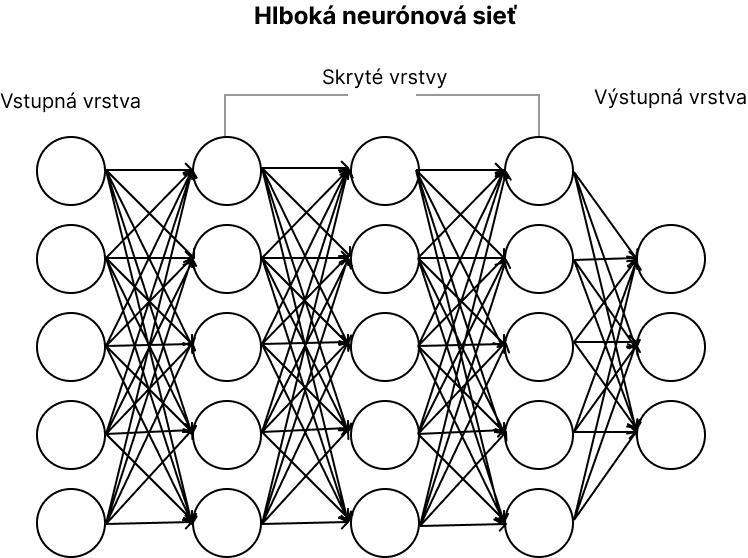
\includegraphics[width=0.5\textwidth]{images/hlboka neur siet.jpg}}
\caption{Ilustrácia hlbokej neurónovej siete s tromi skrytými vrstvami.}
\label{fig:neuron}
\end{figure}

Hlbokú neurónovú sieť z Obr. \ref{fig:neuron} môžeme formálne definovať predpisom:

\begin{equation}
\begin{split}
  f(x_0) = W_0 x + b_0 \\
  f(x_{l+1}) = W_{l+1} g(x_l) + b_{l+1} \\  
\end{split}
\end{equation}

kde $x$ je vstupná hodnota a $x_l$ od nuly sú aktivácie v jednotlivých vrstvách, $W_l$ označuje váhy vo vrstve $l$ a $b_l$ je bias vo vrstve $l$ a $g$ je aktivačná funkcia.

\subsection{Aktivačné Funkcie} \label{sec:aktivacne_funkcie}

Aktivačná funkcia podľa \cite{Goodfellow-et-al-2016} pridáva do neurónovej siete nelinearitu, čo neurónovej sieti umožňuje aproximovať veľkú triedu funkcií. Medzi známe aktivačné funkcie patria napríklad sigmoid, hyperbolický tangens a ReLU (Rektifikovaná lineárna jednotka). Sigmoid je definovaný predpisom \cite{Goodfellow-et-al-2016}:

\begin{equation}
\sigma(x) = \frac{1}{1 + e^{-x}}
\end{equation}

Hyperbolický tangens je definovaný predpisom \cite{Goodfellow-et-al-2016}:

\begin{equation}
f(x) = tanh(x)
\end{equation}

ReLU je definovaný predpisom \cite{Goodfellow-et-al-2016}:

\begin{equation}
f(x) = max(0, x)
\end{equation}

Z pohľadu vlastností jednotlivých spomenutých aktivačných funkcií sa najčastejšie odporúča používať aktivačná funkcia ReLU. ReLU nemení veľkosť vstupu a medzi jej výhody patrí napríklad efektívnosť jej výpočtu.

\subsection{Stratové Funkcie} \label{sec:stratove_funkcie}

Cieľom stratovej funkcie je umožniť trénovanie neurónovej siete v nami zvolenej úlohe.

Podľa článku \cite{takada2023genelive}, kde sa autori zaoberajú podobným problémom ako my, použili ako stratovú funkciu Binary Cross-Entropy (BCE). BCE je definovaná predpisom podľa \cite{Yaoshiang2020ce}:

\begin{equation}
  J_{bce} = -\frac{1}{M}\sum_{m=1}^{M} \left[ y_{m} \log\left( h_{\theta}(x_{m}) \right) + (1 - y_{m}) \log\left( 1 - h_{\theta}(x_{m}) \right) \right]
\end{equation}

kde $M$ je počet trénovacich dát, $y_{m}$ je požadovaná hodnota, $x_m$ je vstupná hodnota a $h_{\theta}$ je model s váhami neurónovej siete $\theta$.

V našom prípade budeme používať ako stratovú funkciu Categorical (kategorickú) Cross-Entropy (CCE). CCE je definovaná predpisom podľa \cite{Yaoshiang2020ce}:
  
\begin{equation} J_{cce}=-\frac {1}{M}\sum \limits _{k=1}^{K} \sum \limits _{m=1}^{M} {y_{m}^{k}\times \log \left ({h_{\theta }\left ({x_{m},k }\right) }\right)}
\end{equation}

kde $M$ je počet trénovacich dát, $K$ je počet tried, $y_{m}^{k}$ je požadovaná hodnota, $x_m$ je vstupná hodnota a $h_{\theta}$ je model s váhami neurónovej siete $\theta$.

\subsection{Spätná propagácia}

Spätná propagácia je algoritmus, ktorý umožňuje vypočítanú chybu na výstupnej vrstve našej siete propagovať naspäť od výstupnej vrstvy až po vstupnú vrstvu.
Vďaka tomuto algoritmu sme schopný vypočítať gradient vzhľadom na nami zvolenú
stratovú funkciu, čo nám umožňuje určiť, ako malá zmena hodnoty neurónu ovplyvňuje
výsledok siete. Na základe tejto informácie vieme aktualizovať parametre siete tak, aby
sme minimalizovali stratovú funkciu. Proces spätnej propagácie zahŕňa niekoľko krokov:

\begin{enumerate}
  \item \textbf{Dopredny vypocet (Forward Pass)} – Vstupné dáta prejdú cez neurónovú sieť od vstupnej vrstvy až po výstupnú vrstvu. Počas tohto prechodu každý neurón v sieti vypočíta váhovanú sumu vstupov, aplikuje aktivačnú funkciu a prenáša svoj výstup na ďalšie neuróny (Obr. \ref{fig:backpropagation} modré šípky).
  \item \textbf{Výpočet chyby} – Porovnajú sa výstupy siete s očakávanými hodnotami v trénovacích dátach a vypočíta sa chyba. Chyba je meraná pomocou tzv. stratovej funkcie, ktorá vyjadruje rozdiel medzi predpovedanými a skutočnými hodnotami.
  \item \textbf{Spätný prechod (Backward Pass)} – Chyba sa potom „spätným prechodom“ prenáša späť cez sieť. Cieľom je určiť, akým spôsobom by sa mali upraviť váhy jednotlivých neurónov, aby sa minimalizovala chyba. Spätný prechod začína pri výstupnej vrstve a postupuje späť cez sieť až po vstupnú vrstvu (Obr. \ref{fig:backpropagation} červené šípky).
  \item \textbf{Aktualizácia váh} – Počas spätného prechodu sa aktualizujú váhy na základe gradientu chyby voči váham. Gradient je vlastne derivácia stratovej funkcie vzhľadom k váham a vyjadruje, akým smerom a o akú veľkosť sa majú váhy aktualizovať.
  \item \textbf{Opakovanie procesu} – Celý tento proces sa opakuje pre jednotlivé trénovacie vzorky v dátovej množine. Cieľom je minimalizovať chybu na trénovacích dátach a dosiahnuť lepšiu schopnosť generalizácie na nových, neznámich dátach.
\end{enumerate}

\begin{figure}[H]
\centerline{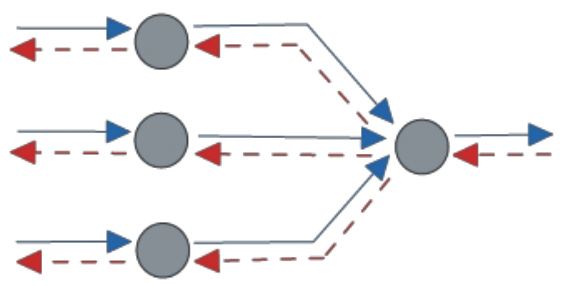
\includegraphics[width=0.5\textwidth]{images/forward_back.png}}
\caption{Princíp spätnej propagácie.}
\label{fig:backpropagation}
\end{figure}

\subsection{Konvolučné neurónové siete}

Pri riešení úloh spojených s počítačovým videním (detekcia objektov, určovanie veku
osôb na obraze, rozpoznávanie tváre...) sa v posledných rokoch stali konvolučné neurónové siete (v literatúre označované aj ako ConvNets alebo CNN) veľmi populárne.
Ide o typ doprednej neurónovej siete, ktorá v oblasti počítačového videnia
pracuje s obrázkami alebo videom (postupnosť obrázkov). Takýto typ dát vieme veľmi
jednoducho reprezentovať pomocou dátovej štruktúry tenzor. V prípade obrázkov ide o
tenzor s rozmerom šírka × výška × hĺbka, kde hĺbka reprezentuje počet kanálov (v prípade RGB obrázkov je počet kanálov 3, naopak šedotónový obraz má kanál iba jeden). Na Obr. \ref{fig:tenzor} môžeme vidieť grafickú reprezentáciu 3 rozmerného tenzora.

\begin{figure}[H]
\centerline{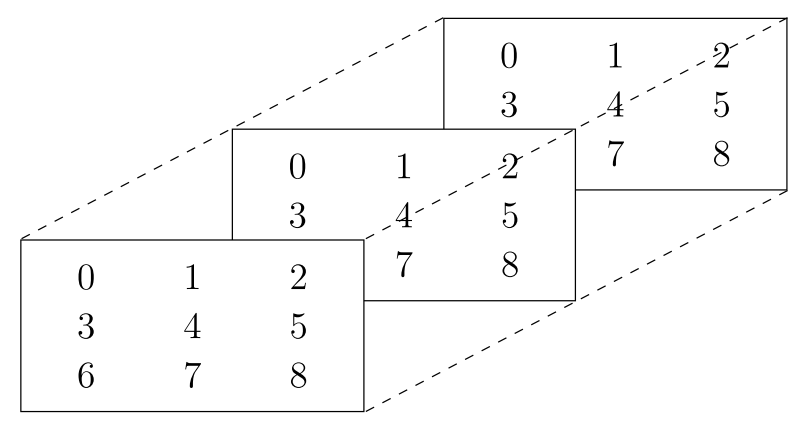
\includegraphics[width=0.5\textwidth]{images/tenzor.png}}
\caption{Ukážka 3 rozmerného (3x3x3) tenzora.}
\label{fig:tenzor}
\end{figure}

Pomocou konvolučných neurónových sietí vieme priradiť dátam význam na základe
vzorov, ktoré vieme získať aplikovaním matematickej operácie konvolúcia. Medzi vzory,
ktoré môžeme získať, patria na vyšších úrovniach rôzne typy hrán a čím ideme vo
vrstvách siete hlbšie, tým vieme získavať komplexnejšie vzory (oči, ucho...) viď Obr. \ref{fig:detekcia_vzorov}.

\begin{figure}[H]
\centerline{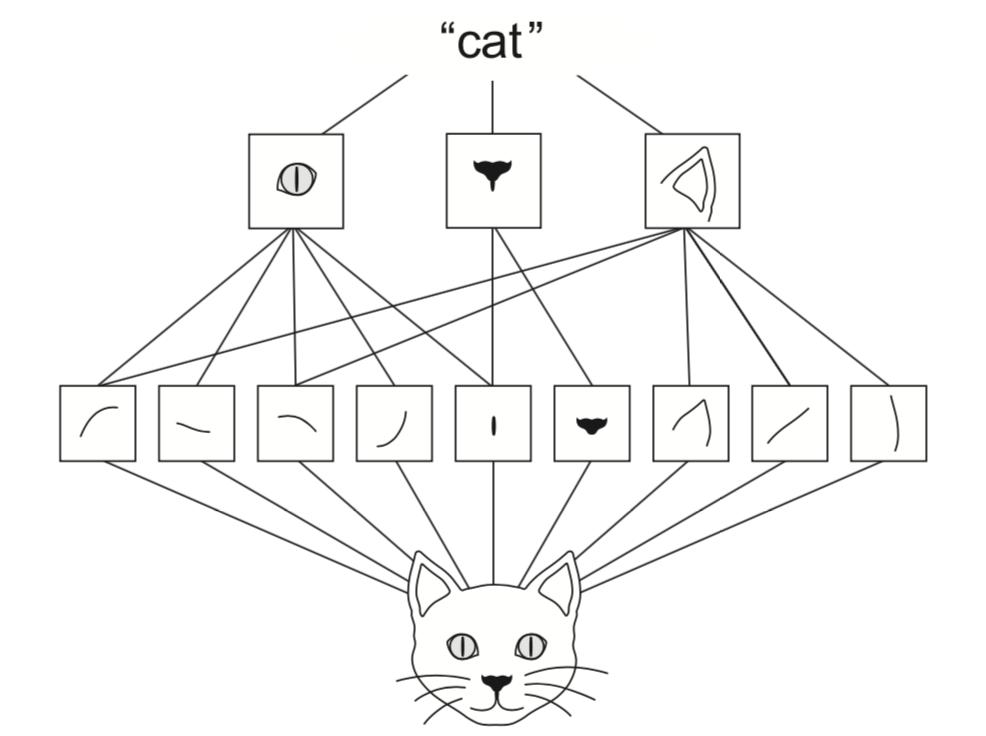
\includegraphics[width=0.5\textwidth]{images/detekcia vzorov.jpg}}
\caption{Príklad detekcie vzorov v konvolučných neurónových sieťach \cite{donahue2017dance}.}
\label{fig:detekcia_vzorov}
\end{figure}

Jednou z hlavných výhod týchto sietí je ekvivariancia voči translácii vstupného
obrazu. Pri vhodne zvolenom postupe trénovania sietí je možné napr. pomocou augmentácie sieť natrénovať tak, aby sa výstup siete nemenil aj pri škálovaní a rotácii
vstupného obrazu. Ďalšie využitie konvolučných neurónových sietí vieme nájsť aj v
spracovaní zvuku alebo v spracovaní prirodzeného jazyka.
Súčasťou architektúr, ktoré využívajú konvolučné neurónové siete sú,
viaceré skryté konvolučné vrstvy, ktoré sa kombinujú s vrstvami, ktoré nazývame pooling vrstvy, aktivačné vrstvy a plne prepojené vrstvy. Príklad architektúry s viacerými
vrstvami môžeme vidieť na Obr. \ref{fig:conv_multi_layer}.

\begin{figure}[H]
\centerline{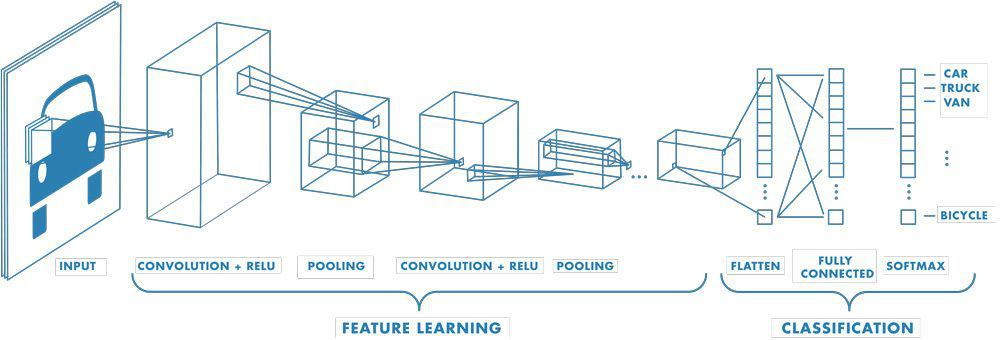
\includegraphics[width=1\textwidth]{images/conv multi layer.jpg}}
\caption{Príklad architektúry konvolučnej neurónovej siete s viacerými vrstvami \cite{convnn}.}
\label{fig:conv_multi_layer}
\end{figure}

\subsection{Konvolučná vrstva}

Táto vrstva pracuje s matematickou operáciou, ktorú nazývame konvolúcia. Konvolúcia je operácia, ktorá pracuje s dvomi funkciami $f$ a $g$ a je definovaná nasledovne:

\begin{equation}
(f * g)(t) = \int_{-\infty}^{\infty} f(x)g(t - x) dx
\end{equation}

V našom prípade si ešte zadefinujeme diskrétnu časť konvolúcie, nakoľko sieť trénujeme
na počítačoch, a tie ako vieme, pracujú s diskrétnymi hodnotami. Konvolúcia je v
diskrétnej verzii definovaná pre $f$ a $g$ nasledovne:

\begin{equation}
(f * g)(t) = \sum_{x=-\infty}^{\infty} f(x)g(t - x)
\end{equation}

Ak pracujeme s obrazom, alebo v našom prípade s audiom vyobrazeným Melovym spektrogramom, tak za funkciu $f$ považujeme vstupný obraz a za funkciu $g$ jadro (taktiež aj kernel). V tomto prípade hovoríme o dvojrozmernej konvolúcii, ktorá
je definovaná predpisom:

\begin{equation}
(f * g)(x, y) = \sum_{i=\infty}^{\infty} \sum_{j=\infty}^{\infty} f(i, j)g(x - i, y - j)
\end{equation}

Výstupom 2 rozmernej konvolúcie je takzvaná mapa príznakov. Konvolučná vrstva znižuje šírku a výšku obrazu oproti vstupu. Grafickú reprezentáciu 2 rozmernej konvolúcie môžeme vidieť na Obr. \ref{fig:2d_konvolucia}.

\begin{figure}[H]
\centerline{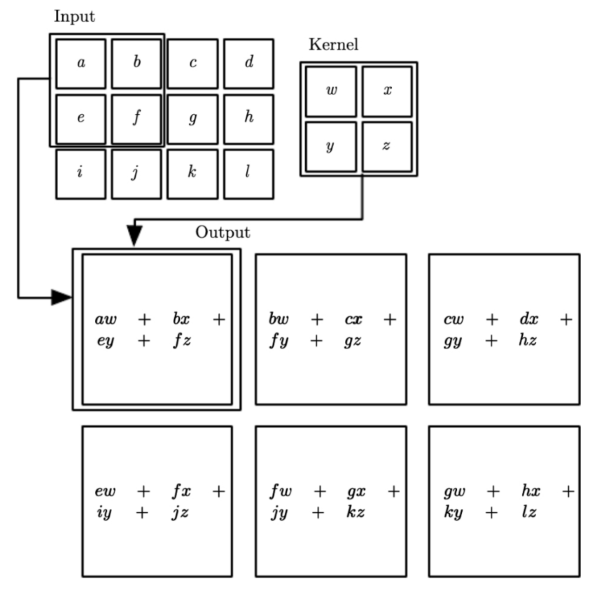
\includegraphics[width=0.75\textwidth]{images/konvolucia.png}}
\caption{Grafická reprezentácia 2 rozmernej konvolúcie \cite{convnn}. Ako môžeme vidieť, na vstupe
sme získali maticu o veľkosti 3×4 a aplikovaním jadra 2×2 sme získali výstupnú mapu
príznakov s rozmerom 2×3.}
\label{fig:2d_konvolucia}
\end{figure}

Výstup konvolučnej vrstvy (mapa príznakov) je následne vstupom pre ďalšiu vrstvu a
to konkrétne aktivačnú vrstvu.

\subsection{Aktivačná vrstva}

Úlohou aktivačnej vrstvy je pridávanie nelinearity na mapu príznakov
z konvolučnej vrstvy za pomoci vhodnej aktivačnej funkcie. Pri konvolučných neurónových sieťach je najčastejšie ako aktivačná funkcia používaná ReLU (Rektifikovaná lineárna jednotka).

Ak by sme vynechali túto vrstvu (pridanie aktivačnej funkcie), tak by sa naša sieť
v priebehu trénovania nedokázala zlepšovať a stal by sa z nej iba lineárny klasifikátor.
Výstup z aktivačnej vrstvy je následne vstupom pre pooling vrstvu.

\subsection{Pooling vrstva}

Problémom mapy príznakov z predchádzajúcich vrstiev je citlivosť na pozíciu príznakov
v obraze. To znamená, že zmena veľkosti, otočenie alebo posun môžu výrazne zmeniť
výslednú mapu príznakov. O riešenie tohto problému sa stará pooling vrstva a to tak, že
zmenšuje mapu príznakov. Týmto prístupom zaručíme, že ďalšie vrstvy sa budú pozerať už iba na najvýznamnejšie príznaky a tie menej dôležité (akými sú napríklad veľmi podrobné detaily), sa znížením rozmerov odstránia. Ďalšími výhodami tejto vrstvy sú
zníženie počtu trénovacích parametrov, čo znižuje počet výpočtov, a teda aj času potrebného pre trénovanie siete a predchádza javu, ktorý nazývame overfitting (sieť je až veľmi dobré natrénovaná na trénovacích dátach). Najznámejšie funkcie využívané pre
operáciu poolingu sú max pooling a priemerovací pooling.

Princípom max poolingu je výber maximálnej hodnoty podľa zvoleného rozmeru
filtra Zvyčajne sa volí veľkosť filtra 2×2. Princíp max poolingu môžeme vidieť
na Obr. \ref{fig:max_pooling}.

\begin{figure}[H]
\centerline{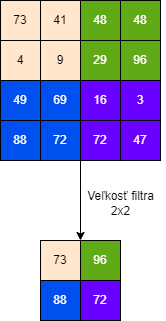
\includegraphics[width=0.25\textwidth]{images/max pool.drawio.png}}
\caption{Príklad max poolingu.}
\label{fig:max_pooling}
\end{figure}

Princípom priemerovacieho poolingu je výber priemeru hodnôt podľa zvoleného rozmeru filtra. Zvyčajne sa volí veľkosť filtra 2×2. Princíp priemerovacieho poolingu môžeme vidieť na Obr. \ref{fig:avg_pooling}.

\begin{figure}[H]
\centerline{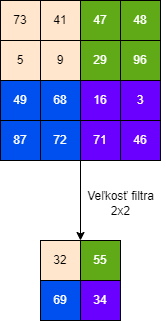
\includegraphics[width=0.25\textwidth]{images/avgpool.drawio.png}}
\caption{Príklad priemerovacieho poolingu.}
\label{fig:avg_pooling}
\end{figure}

Po poslednej pooling vrstve väčšinou nasleduje plne prepojená vrstva. Vstupom pre
plne prepojenú vrstvu nie je ale tenzor vyššieho rádu, ale iba tenzor prvého rádu. Z
tohto dôvodu potrebujeme na výstup poslednej pooling vrstvy aplikovať jednu z nasledujúcich operácií, a to buď operáciu flatten alebo globálny pooling.


Princípom operácie flatten je vytvoriť tenzor prvého rádu pomocou sploštenia viacrozmerného vstupného tenzora. Výstupom operácie flatten bude teda tenzor s počtom prvkov podľa vzorca (\ref{eq:flatten}), kde $x$ počet prvkov výstupného tenzoru, $n$ je rád tenzoru
a $S_i$ je veľkosť dimenzie $i$.

\begin{equation}
x = \prod_{i=1}^{n} S_i
\label{eq:flatten}
\end{equation}

Ilustráciou operácie flatten môžeme vidieť na Obr. \ref{fig:flatten}.

\begin{figure}[H]
\begin{align*}
  \begin{bmatrix}
      1 & 2 & 3 \\
      4 & 5 & 6 \\
      7 & 8 & 9 \\
  \end{bmatrix}
  \longrightarrow 
  &
  \begin{bmatrix}
      1 \\
      2 \\
      3 \\
      4 \\
      5 \\
      6 \\
      7 \\
      8 \\
      9 \\
  \end{bmatrix}
\end{align*}
\caption{Ilustrácia operácie flatten.}
\label{fig:flatten}
\end{figure}

V praxi sa ale odporúča využívať namiesto operácie flatten globálny pooling. Princípom globálneho poolingu je aplikovať pooling pozdĺž dimenzií, ktoré reprezentujú
výšku a šírku príznakových máp vstupného tenzora. Výsledný tenzor prvého
rádu bude mať teda taký počet prvkov, koľko kanálov mal vstupný tenzor. Ilustráciu
globálneho priemerovacieho poolingu (GPP) môžeme vidieť na Obr. \ref{fig:gap}.

\begin{figure}[H]
  \centerline{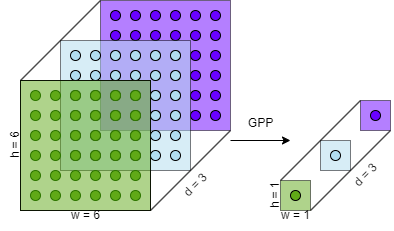
\includegraphics[width=0.5\textwidth]{images/gap.drawio.png}}
  \caption{Ilustrácia globálneho priemerovacieho poolingu.}
  \label{fig:gap}
\end{figure}

Po aplikácii operácie flatten alebo globálneho priemerovacieho poolingu po poslednej pooling vrstve je tenzor prvého rádu vstupom pre plne prepojenú vrstvu.

\subsection{Plne prepojená vrstva}

Poslednou fázou v konvolučných neurónových sieťach väčšinou býva plne prepojená
vrstva. Ako už názov tejto vrstvy napovedá, všetky neuróny tejto vrstvy sú navzájom
plne prepojené ako tomu je aj v klasických neurónových sieťach. Úlohou tejto vrstvy je
na základe príznakov naučených z predchádzajúcich vrstiev zaradiť objekt, ktorý bol
na vstupnom obraze do správnej výstupnej triedy.